\documentclass[12pt, a4paper]{article}
\usepackage[utf8]{inputenc}
\usepackage{listings}
\usepackage{color}
\usepackage[pdftex]{graphicx}     
\usepackage{subcaption}
\usepackage{graphicx}
\usepackage{grffile}

\linespread{1.3}
\setlength{\parindent}{4em}
\definecolor{codegreen}{rgb}{0,0.6,0}
\definecolor{codegray}{rgb}{0.5,0.5,0.5}
\definecolor{codepurple}{rgb}{0.58,0,0.82}
\definecolor{backcolour}{rgb}{0.95,0.95,0.92}
 
\lstdefinestyle{mystyle}{
    rulesepcolor=\color{magenta},
    commentstyle=\color{codegreen},
    keywordstyle=\color{magenta},
    stringstyle=\color{codepurple},
    basicstyle=\footnotesize,
    breakatwhitespace=false,         
    breaklines=true,                 
    captionpos=b,                    
    keepspaces=false,                 
    showspaces=false,  
    showstringspaces=false,
    showtabs=false,                  
    xrightmargin=10 pt,
}
\title{\vspace*{2 in}ADA Laboratory Record}
\author{Dinesh K R Navada\\1SI16CS034}
\date{}
\begin{document}
\pagenumbering{gobble}
%\tableofcontents
%\newpage
\maketitle
\newpage
\pagenumbering{arabic}
\lstset{numbers=left, numberstyle=\tiny, stepnumber=1, numbersep=5 pt}
\lstset{style=mystyle,
basicstyle=\linespread{1.1}\fontsize{9}{13}\selectfont\ttfamily,literate={\	}{{\ }}4}
\section{Divide and conquer}\subsection*{Problem Statement:}\par\textit{Use divide and conquer method to recursively implement the following \\algorithms.\\\textbf{a.}
 Binary Search and Linear Search.\\
\textbf{b.} To find the maximum and minimum in a given list of n elements.}
\subsection*{Solution}
\subsubsection*{1.c.Maximum and Minimum elements}
\lstinputlisting[language=C]{"./Implementation/MaxMin.c"}
\newpage
\subsubsection*{Output}
\begin{figure*}[h]
\centering
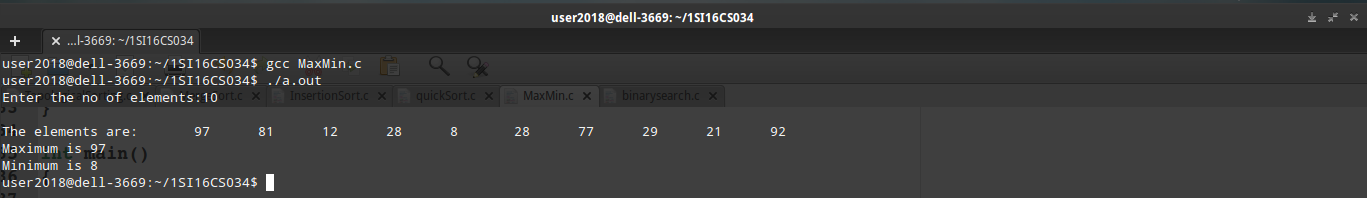
\includegraphics[width=5 in,height=1.3 in]{./Output/im1.png}
\label{Figure 2}
\caption{Case 1}
\end{figure*}
\begin{figure*}[h]
\centering
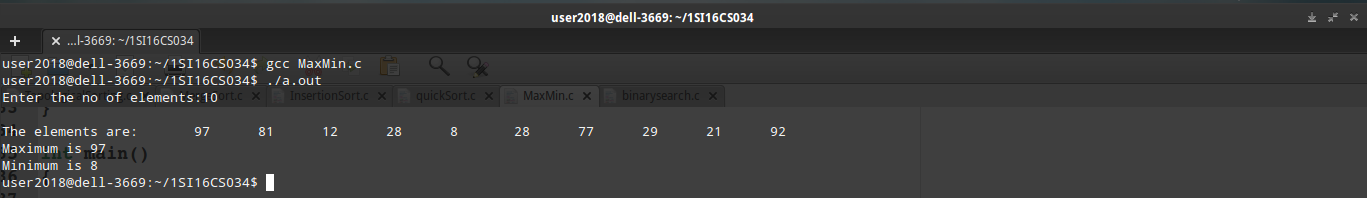
\includegraphics[width=5 in,height=1.3 in]{./Output/im2.png}
\label{Figure 3}
\caption{Case 2}
\end{figure*}
\newpage
\subsubsection*{2.Insertion Sort}
\lstinputlisting[language=C]{"./Implementation/InsertionSort.c"}
\subsubsection*{Output}
\begin{figure*}[h]
\centering
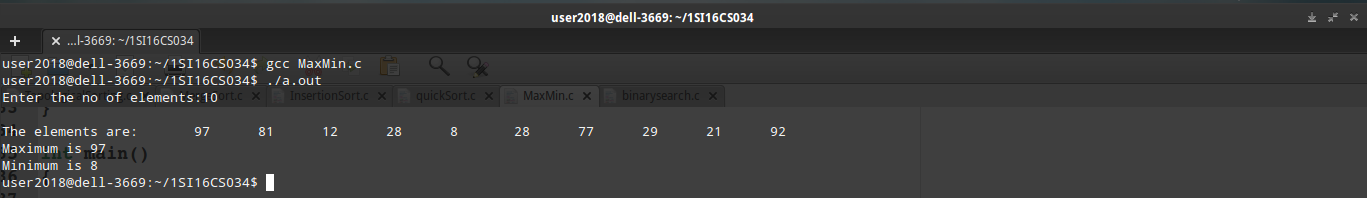
\includegraphics[width=5 in,height=2 in]{./Output/im1.png}
\label{Figure 2}
\caption{Case 1}
\end{figure*}
\begin{figure*}[h]
\centering
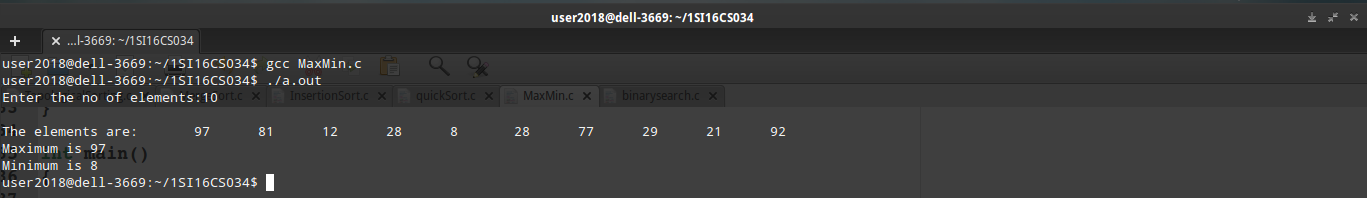
\includegraphics[width=5 in,height=2 in]{./Output/im2.png}
\label{Figure 3}
\caption{Case 2}
\end{figure*}

\section{Merge Sort}\subsection*{Problem Statement:}\par\textit{Sort a given set of elements using the Merge sort method and determine the time
required to sort the elements. Repeat the experiment for different values of n, the
number of elements in the list to be sorted and plot a graph of the time taken
versus n. The elements can be read from a file or can be generated using the
random number generator.}
\subsection*{Solution}
\lstinputlisting[language=C]{"./Implementation/MergeSort.c"}
\subsection*{Efficiency}
\begin{figure*}[h]
\centering
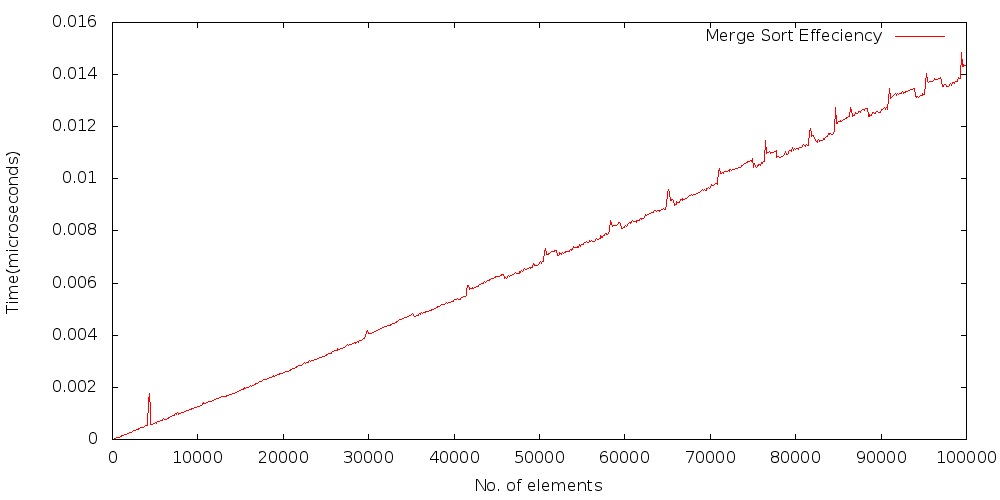
\includegraphics[width=5 in]{./Performance_graphs/mergeplot.png}
\label{Figure 1}
\caption{Plot of Time(Y-axis) v/s No. of elements(X-axis)}
\end{figure*}
\newpage
\subsection*{Output}
\begin{figure*}[h]
\centering
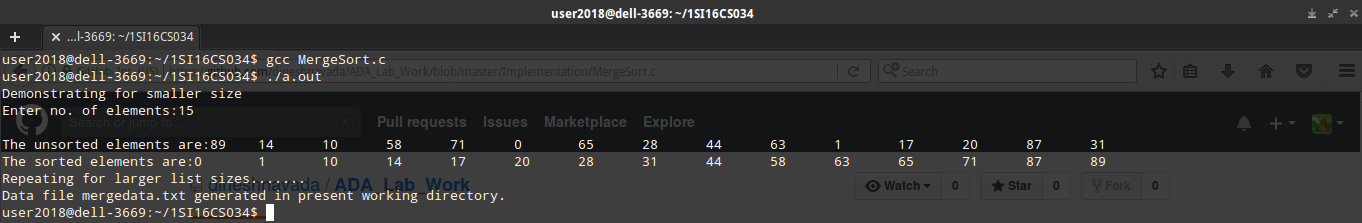
\includegraphics[width=5.2 in,height=2.5 in]{./Output/im5.png}
\label{Figure 2}
\caption{Case 1}
\end{figure*}
\begin{figure*}[h]
\centering
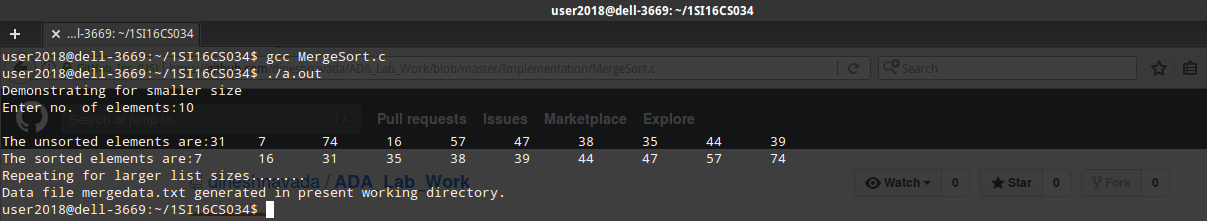
\includegraphics[width=5.2 in,height=2.5 in]{./Output/im6.png}
\label{Figure 3}
\caption{Case 2}
\end{figure*}
\newpage
\section{Quick Sort}\subsection*{Problem Statement:}\par\textit{Sort a given set of elements using the Quick sort method and determine the time
required to sort the elements. Repeat the experiment for different values of n, the
number of elements in the list to be sorted and plot a graph of the time taken
versus n. The elements can be read from a file or can be generated using the
random number generator.}
\subsection*{Solution}
\lstinputlisting[language=C]{"./Implementation/quickSort.c"}
\subsection*{Efficiency}
\begin{figure*}[h]
\centering
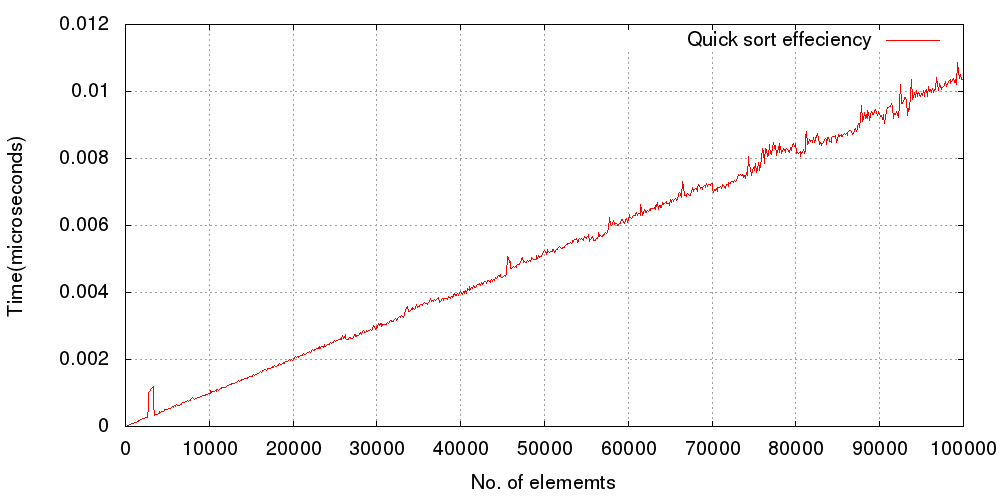
\includegraphics[width=5 in]{./Performance_graphs/quick.png}
\label{Figure 1}
\caption{Plot of Time(Y-axis) v/s No. of elements(X-axis)}
\end{figure*}
\newpage
\subsection*{Output}
\begin{figure*}[h]
\centering
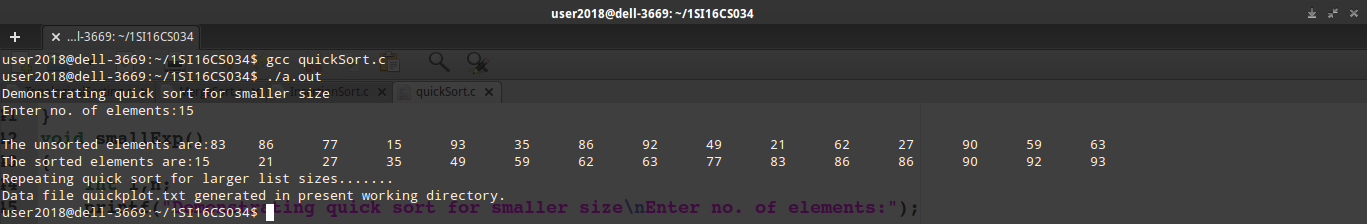
\includegraphics[width=5.3 in,height=2.5 in]{./Output/im3.png}
\label{Figure 2}
\caption{Case 1}
\end{figure*}
\begin{figure*}[h]
\centering
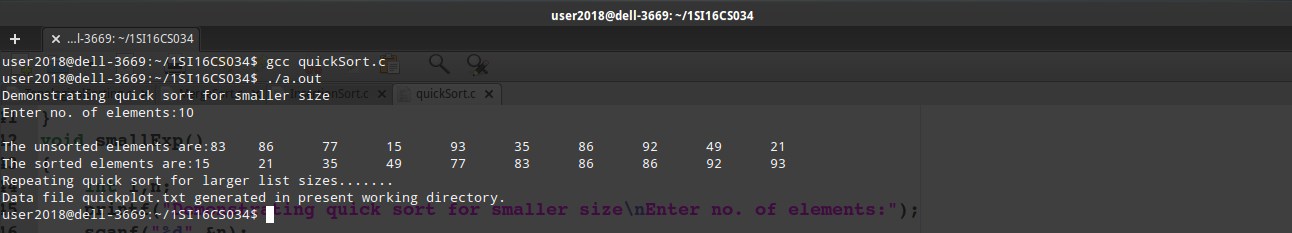
\includegraphics[width=5.3 in,height=2.5 in]{./Output/im4.png}
\label{Figure 3}
\caption{Case 2}
\end{figure*}
\newpage
\section{Decrease and conquer}\subsection*{Problem Statement:}\par\textit{\textbf{a.} Obtain the Topological ordering of vertices in a given digraph.\\
\textbf{b.} Sort a given set of elements using Insertion sort method.}
\subsection*{Solution}
\subsubsection*{1.Topological Ordering}
\lstinputlisting[language=C]{"./Implementation/TopologicalSorting.c"}
\subsubsection*{Input Graphs}
\begin{figure*}[h]
\centering
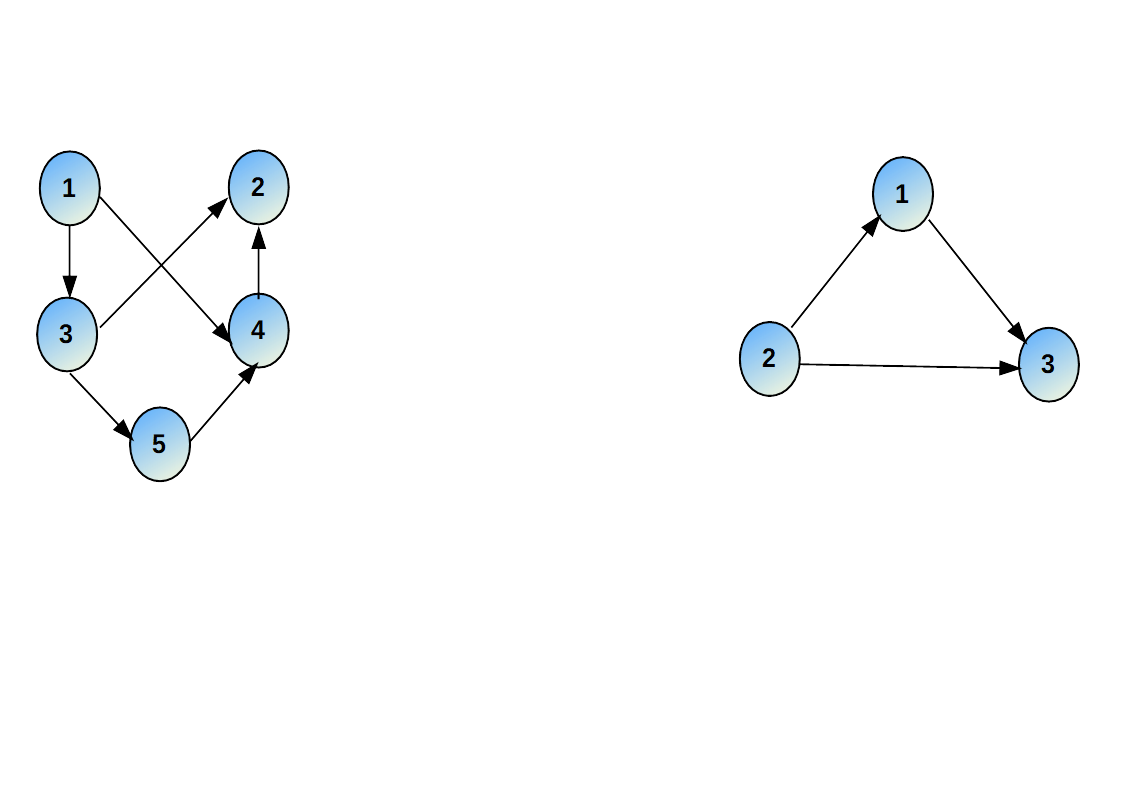
\includegraphics[width=3.5 in,height=2 in]{./Output/TopologicalSortIn.png}
\label{Figure 2}
\caption{Input graphs}
\end{figure*}
\newpage
\subsubsection*{Output}
\begin{figure*}[h]
\centering
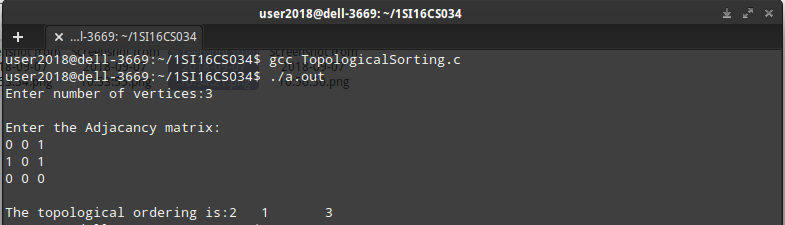
\includegraphics[width=5 in,height=2.5 in]{./Output/im9.png}
\label{Figure 2}
\caption{Case 1}
\end{figure*}
\begin{figure*}[h]
\centering
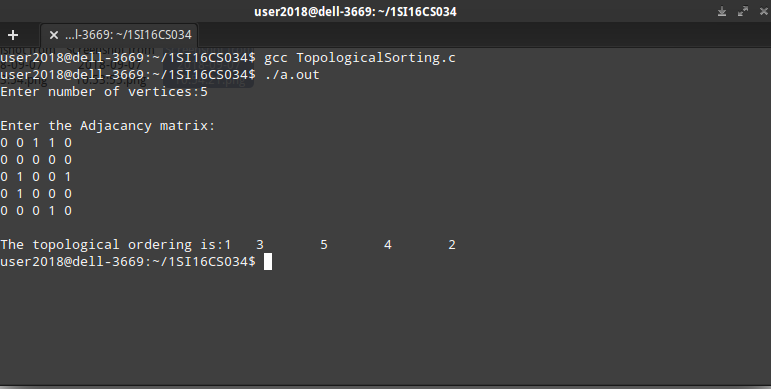
\includegraphics[width=5 in,height=2.5 in]{./Output/im10.png}
\label{Figure 3}
\caption{Case 2}
\end{figure*}
\newpage
\subsubsection*{2.Insertion Sort}
\lstinputlisting[language=C]{"./Implementation/InsertionSort.c"}
\subsubsection*{Output}
\begin{figure*}[h]
\centering
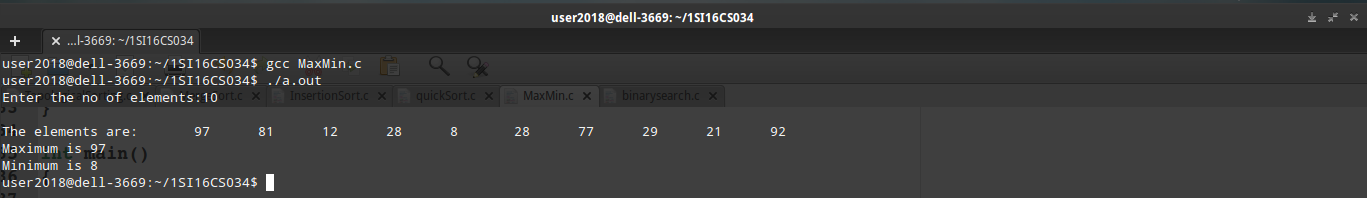
\includegraphics[width=5 in,height=2 in]{./Output/im1.png}
\label{Figure 2}
\caption{Case 1}
\end{figure*}
\begin{figure*}[h]
\centering
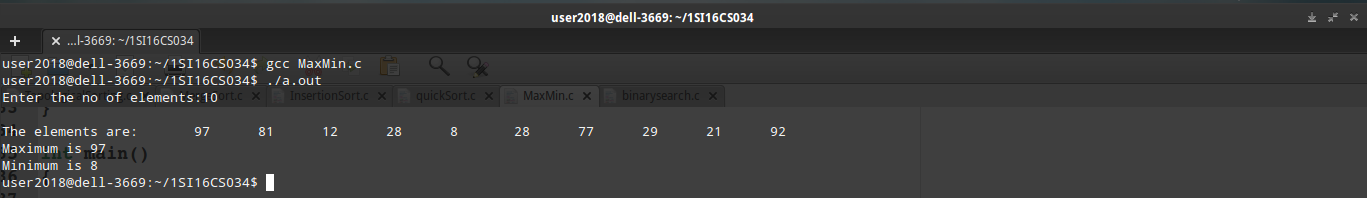
\includegraphics[width=5 in,height=2 in]{./Output/im2.png}
\label{Figure 3}
\caption{Case 2}
\end{figure*}
\end{document}